% -*- coding: utf-8-unix -*- 
% === Einheit ====================================================================
%\Tut\chapter{Graphen}
\begin{extract*}
  \chapter{Graphen}
\end{extract*}
\label{k:graphen} 

\begin{extract}
  \begin{center}\Large\bfseries Hinweise f\"ur die Tutorien\end{center}
\end{extract}

In den bisherigen Einheiten kamen schon an mehreren Stellen Diagramme
und Bilder vor, in denen irgendwelche "`Gebilde"' durch Linien oder
Pfeile miteinander verbunden waren.
% 
Man erinnere sich etwa an die Ableitungsbäume wie in
Abbildung~\ref{fig:abl-baum-informell} in der
\hyperref[k:grammatiken]{Einheit über Grammatiken}, an Huffman-Bäume
wie in Abbildung~\ref{abb:huffman-baum} der
\hyperref[k:codierungen]{Einheit über Codierungen}, oder an die
Abbildung am Ende von Abschnitt~\ref{sub:information}.

Das sind alles Darstellungen sogenannter Graphen.
% 
Sie werden in dieser Einheit sozusagen vom Gebrauchsgegenstand zum
Untersuchungsgegenstand.
% 
Dabei unterscheidet man üblicherweise gerichtete und ungerichtete
Graphen, denen im folgenden getrennte Abschnitte gewidmet sind.

%-----------------------------------------------------------------------
%%\Tut\section{Gerichtete Graphen}
\begin{extract*}
  \section{Gerichtete Graphen}
\end{extract*}
\label{sub:digraph}

%-----------------------------------------------------------------------
%\Tut\subsection{Graphen und Teilgraphen}
\begin{extract*}
  \subsection{Graphen und Teilgraphen}
\end{extract*}
\label{subsub:graphen-teilgraphen}

Ein \mdefine{gerichteter\\Graph}\index{Graph!gerichtet}%
\index{gerichteter Graph} ist festgelegt durch ein Paar $G=(V,E)$,
wobei $E\subseteq V\x V$ ist.
% 
Die Elemente von $V$ heißen \mdefine{Knoten}, die Elemente von $E$
heißen \mdefine{Kanten}. Wir verlangen (wie es üblich ist), dass die
Knotenmenge nicht leer ist.
% 
Und wir beschränken uns in dieser Vorlesung auf \emph{endliche}
Knotenmengen. Die Kantenmenge darf leer sein.

Typischerweise stellt man Graphen graphisch dar.
% 
Statt zu schreiben
% 
\begin{align*} V &= \{ 0,1,2,3,4,5 \} \\ E &= \{ (0,1), (0,3), (1,2),
(1,3), (4,5), (5,4) \}
\end{align*}
% 
malt man lieber Abbildungen wie diese:
% 
\begin{figure}[ht] \hbox to \textwidth{
    \begin{tikzpicture}[->,>=stealth] \matrix [matrix of math
nodes,nodes={circle,draw,minimum size=5mm,inner sep=2pt},row
sep=10mm,column sep=10mm] { |(0)| & |(1)| & |(2)| \\ |(3)| & |(4)| &
|(5)| \\ }; \draw (0) -- (1); \draw (0) -- (3); \draw (1) -- (2);
\draw (1) -- (3); \draw (4) to [bend left] (5); \draw (5) to [bend
left] (4);
    \end{tikzpicture} \hss
    \begin{tikzpicture}[->,>=stealth] \matrix [matrix of math
nodes,nodes={circle,draw,minimum size=5mm,inner sep=2pt},row
sep=10mm,column sep=10mm] { |(0)| 0 & |(1)| 1 & |(2)| 2 \\ |(3)| 3 &
|(4)| 4 & |(5)| 5 \\ }; \draw (0) -- (1); \draw (0) -- (3); \draw (1)
-- (2); \draw (1) -- (3); \draw (4) to [bend left] (5); \draw (5) to
[bend left] (4);
    \end{tikzpicture} }
  \caption{zweimal der gleiche Graph: links ohne Angabe der
Knotenidentitäten, rechts mit}
  \label{abb:graph-ohne-mit}
\end{figure}

\noindent Ob man die Knoten als anonyme dicke Punkte oder Kringel
darstellt wie auf der linken Seite in
Abbildung~\ref{abb:graph-ohne-mit}, oder ob man jeweils das
entsprechende Element von $V$ mit notiert wie auf der rechten Seite in
Abbildung~\ref{abb:graph-ohne-mit}, hängt von den Umständen ab. Beides
kommt vor.
% 
Eine Kante $(x,y)$ wird durch einen Pfeil von dem Knoten $x$ in
Richtung zu dem Knoten $y$ dargestellt.
% 
Wenn es eine Kante $(x,y)\in E$ gibt, dann sagt man auch, die Knoten
$x$ und $y$ seien \mdefine[adjazente
Knoten]{adjazent}\index{Knoten!adjazente}\index{adjazente Knoten}.
% 
Man beachte aber, diese Relation nicht symmetrisch ist, obwohl die
Formulierung es suggeriert! % TODO: Symmetrie schon definiert???

Außerdem ist die Anordnung der Knoten in der Darstellung irrelevant.
Abbildung~\ref{abb:graph-mit-2} zeigt den gleichen Graphen wie
Abbildung~\ref{abb:graph-ohne-mit}:

\begin{figure}[ht] \centering
  \begin{tikzpicture}[->,>=stealth] \matrix [matrix of math
nodes,nodes={circle,draw,minimum size=5mm,inner sep=2pt},row
sep=10mm,column sep=10mm] { |(1)| 1 & & |(2)| 2 & |(4)| 4 \\ & |(3)| 3
& |(0)| 0 & |(5)| 5 \\ }; \draw (0) -- (1); \draw (0) -- (3); \draw
(1) -- (2); \draw (1) -- (3); \draw (4) to [bend left] (5); \draw (5)
to [bend left] (4);
  \end{tikzpicture}
  \caption{eine andere Zeichnung des Graphen aus
Abbildung~\ref{abb:graph-ohne-mit}}
  \label{abb:graph-mit-2}
\end{figure}

\noindent Wir wollen noch zwei weitere Beispiele betrachten.
% 
Im ersten sei $G=(V,E)$ definiert durch
\begin{itemize}
\item $V=\{\#1\}\left(\bigcup_{i=0}^2 \{\#0,\#1\}^i\right)$ und
\item $E=\{ (w,wx) \mid x\in \{\#0,\#1\}\land w\in V \land wx\in V
\}$.
\end{itemize}
% 
Schreibt man die beiden Mengen explizit auf, ergibt sich
\begin{itemize}
\item $V = \{ \#1, \#{10}, \#{11}, \#{100}, \#{101}, \#{110}, \#{111}
\}$
\item $E = \{ (\#1,\#{10}), (\#1,\#{11}), (\#{10},\#{100}),
(\#{10},\#{101}), (\#{11},\#{110}), (\#{11},\#{111}) \}$
\end{itemize}
% 
Im einem Bild kann man diesen Graphen so hinmalen:

\begin{figure}[ht] \centering
  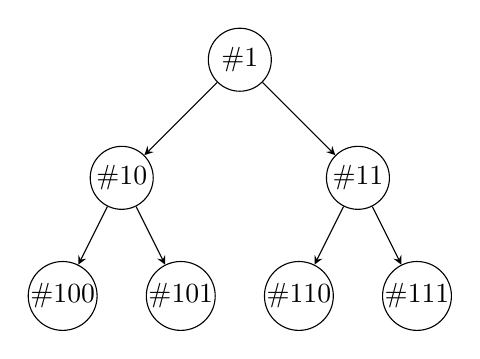
\begin{tikzpicture} [level 1/.style={sibling distance=30mm}, level
2/.style={sibling distance=30mm}, level 3/.style={sibling
distance=10mm}, nodes={draw,circle,inner sep=0pt, minimum size=8mm},
->,>=stealth]
    
    \node {$\#1$} child { node {$\#{10}$} edge from parent [level
2/.style={sibling distance=15mm}] child {node {$\#{100}$} edge from
parent } child {node {$\#{101}$} edge from parent} } child { node
{$\#{11}$} edge from parent [level 2/.style={sibling distance=15mm}]
child {node {$\#{110}$} edge from parent } child {node {$\#{111}$}
edge from parent } } ;
  \end{tikzpicture}
  \caption{ein Graph, der ein sogenannter Baum ist}
  \label{abb:baum}
\end{figure}
% 
Als zweites Beispiel wollen wir den Graphen $G=(V,E)$ betrachten, für
den gilt:
\begin{itemize}
\item $V=\{\#0,\#1\}^3$
\item $E=\{ (xw,wy) \mid x,y\in \{\#0,\#1\}\land w\in \{\#0,\#1\}^2
\}$
\end{itemize}
% 
Die Knotenmenge ist also einfach $V = \{ \#{000}$, $\#{001}$,
$\#{010}$, $\#{011}$, $\#{100}$, $\#{101}$, $\#{110}$, $\#{111} \}$.
% 
Die Kantenmenge wollen wir gar nicht mehr vollständig aufschreiben.
% 
Nur zwei Kanten schauen wir uns beispielhaft kurz an:
\begin{itemize}
\item Wählt man $x=y=\#0$ und $w=\#{00}$ dann ist laut Definition von
$E$ also $(\#{000},\#{000})$ eine Kante.
\item Wählt man $x=\#0$, $y=\#1$ und $w=\#{10}$ dann ist laut
Definition von $E$ also $(\#{010},\#{101})$ eine Kante.
\end{itemize}
% 
Graphisch kann man diesen Graphen \zB wie in
Abbildung~\ref{abb:debruijn} darstellen.
% 
Es handelt sich um einen sogenannten De Bruijn"=Graphen.
\begin{figure}[ht]
  \centering
  \begin{tikzpicture}
    \matrix[matrix of math nodes,nodes={circle,draw,inner sep=0pt, minimum size=8mm},row sep=5mm,column sep=5mm] {
      & 
      |(001)| \#{001}  &
      &
      & 
      & 
      |(011)| \#{011} &
      \\
      |(000)| \#{000}  & 
      &
      |(010)| \#{010} &
      & 
      |(101)| \#{101}  &
      & 
      |(111)| \#{111} \\
      & 
      |(100)| \#{100}  &
      &
      & 
      & 
      |(110)| \#{110} &
      \\
    };
    \begin{scope}[->,>=stealth]
      \draw (000) to [bend left] (001);
      \draw (001) to [bend left] (010);
      \draw (010) to [bend left] (100);
      \draw (100) to [bend left] (000);

      \draw (010) to [bend left] (101);
      \draw (101) to [bend left] (010);

      \draw (111) to [bend left] (110);
      \draw (110) to [bend left] (101);
      \draw (101) to [bend left] (011);
      \draw (011) to [bend left] (111);

      \draw (001) -- (011);
      \draw (110) -- (100);
      \draw (100) -- (001);
      \draw (011) -- (110);

      \path (000) edge [loop left] ();
      \path (111) edge [loop right] ();

    \end{scope}
  \end{tikzpicture}
  \caption{Der de Bruijn-Graphen mit 8 Knoten}
  \label{abb:debruijn}
\end{figure}
% 
Wie man sieht, können bei einer Kante Start- und Zielknoten gleich
sein.
% 
Eine solche Kante, die also von der Form $(x,x)\in E$ ist, heißt auch
eine \mdefine{Schlinge}\index{Schlinge}.
% 
Manchmal ist es bequem, davon auszugehen, dass ein Graph keine
Schlingen besitzt.
% 

Ein solcher Graph heißt \mdefine{schlingenfrei}\index{schlingenfreier
Graph}\index{Graph!schlingenfrei}.

% --------------------------------------------------------------
\begin{tutorium}
  \paragraph{Graphen:}
  \begin{itemize}
  \item zur Motivation:
    \begin{itemize}
    \item Einbahnstraßensystem, .....
    \item wie würde man Zweibahnstraßen modellieren? die Fahrspuren
      für beide Richtungen separat
    \item \textbf{Achtung:} analoge Idee für Autobahmodellierung
      (mehrere Spuren in die gleiche Richtung zwischen zwei Knoten)
      geht nicht: $E\subseteq V\x V$ erlaubt nur: es gibt \emph{keine}
      Kante von $x$ nach $y$ oder es gibt \emph{eine} Kante.
      sogenannte Mehrfachkanten sind bei uns nicht möglich.
    \end{itemize}
  \item Beispiele malen:
    \begin{itemize}
    \item einschließlich Extremfälle mit $0$ Kanten \bzw maximal
      vielen Kanten; mit Schlingen und ohne Schlingen.
    \item Sonderfälle wie Bäume (siehe weiter unten) und Zyklen
    \item Beim Malen darauf hinweisen, dass man den gleichen Graphen
      unterschiedlich hinmalen kann, \zB den $K_4$ mit sich kreuzenden
      Kanten oder ohne.
    \end{itemize}
  \item Eigenschaften von Graphen an Beispielen diskutieren
    \begin{itemize}
    \item beim Straßensystem: Man möchte von jedem Knoten zu jedem
      kommen.
    \item Wenn die Knoten Rechner sind und die Kanten Kabel: Man
      möchte von $x$ nach $y$ nur über möglichst "`wenige"' Kanten
      laufen müssen (egal wo $x$ und $y$)
    \item Wenn die Knoten Rechner sind und die Kanten Kabel: es sollen
      viele gleichzeitig Daten austauschen können: von einer Hälfte in
      die andere möglichst viele Kanten (egal welche Knoten in der
      einen Hälfte sind und welche in der anderen)
    \end{itemize}
  \item Wenn ein Graph $n$ Knoten hat:
    \begin{itemize}
    \item Wieviele Kanten kann er maximal haben, wenn Schlingen
      erlaubt sind? $n^2$ \\ Begründung: klar
    \item Wieviele Kanten kann er maximal haben, wenn er schlingenfrei
      ist? $n(n-1)$ \\ Begründung: $n^2-n$
    \end{itemize}
  \end{itemize}
\end{tutorium}
%----------------------------------------------------------------

Ein ganz wichtiger Begriff ist der eines Teilgraphen eines gegebenen
Graphen.
% 
Wir sagen, dass $G'=(V',E')$ ein \mdefine{Teilgraph}\index{Teilgraph}
von $G=(V,E)$ ist, wenn $V'\subseteq V$ ist und $E'\subseteq E \cap
V'\x V'$.
% 
Knoten- und Kantenmenge von $G'$ müssen also Teilmenge von $V$ \resp
$E$ sein, und die Endpunkte jeder Kante von $E'$ müssen auch zu $V'$
gehören.

Als Beispiel zeigen wir einen Teilgraphen des oben dargestellten de
Bruijn-Graphen:

\begin{figure}[ht]
  \centering
  \begin{tikzpicture}
    \matrix[matrix of math nodes,nodes={circle,draw,inner sep=0pt, minimum size=8mm},row sep=5mm,column sep=5mm] {
      & 
      |(001)| \#{001}  &
      &
      & 
      & 
      |(011)| \#{011} &
      \\
      |(000)| \#{000}  & 
      &
      & %|(010)| \#{010} &
      & 
      |(101)| \#{101}  &
      & 
      |(111)| \#{111} \\
      & 
      |(100)| \#{100}  &
      &
      & 
      & 
      |(110)| \#{110} &
      \\
    };
    \begin{scope}[->,>=stealth]
      \draw (000) to [bend left] (001);
      %\draw (001) to [bend left] (010
      %\draw (010) to [bend left] (100);
      \draw (100) to [bend left] (000);

      %\draw (010) to [bend left] (101);
      %\draw (101) to [bend left] (010);

      %\draw (111) to [bend left] (110);
      \draw (110) to [bend left] (101);
      \draw (101) to [bend left] (011);
      \draw (011) to [bend left] (111);

      %\draw (001) -- (011);
      %\draw (110) -- (100);
      \draw (100) -- (001);
      \draw (011) -- (110);

      %\path (000) edge [loop left] ();
      \path (111) edge [loop right] ();

    \end{scope}
  \end{tikzpicture}
  \caption{Ein Teilgraph des de Bruijn-Graphen aus Abbildung~\ref{abb:debruijn}}
  \label{abb:teilgraph}
\end{figure}
% 
% --------------------------------------------------------------
\begin{tutorium}
  \paragraph{Definition Teilgraph:}
  \begin{itemize}
  \item Beachte: zu jeder Kante, die man in $E'$ haben will, müssen
auch Anfangs- und Endknoten in $V'$ vorhanden sein!
  \item hinreichend großes Beispiel machen, bei dem sowohl
$(\{0,1,2\},$ $\{(0,1),(0,2)\})$ als auch
$(\{3,4,5\},\{(3,4),(3,5))\})$ Teilgraph ist:
    \begin{itemize}
    \item \textbf{Achtung:} formal sind das verschiedene
(Teil-)Graphen
    \item \textbf{aha:} aber sie sehen gleich aus: so was nennt man
isomorphe Graphen (ohne dass wir das an dieser Stelle schon
formalisieren wollen)
    \end{itemize}
  \end{itemize}
\end{tutorium}
% ----------------------------------------------------------------------
%\Tut\subsection{Pfade und Erreichbarkeit}
\begin{extract*}
  \subsection{Pfade und Erreichbarkeit}
\end{extract*}
\label{subsub:pfade-erreichbarkeit}

Im folgenden benutzen wir die Schreibweise $M^{(+)}$ für die Menge
aller nichtleeren Listen, deren Elemente aus $M$ stammen.
% 
Und solch eine Liste notieren wir in der Form $(m_1,m_2\,\dots, m_k)$.

Ein weiteres wichtiges Konzept sind Pfade.
% 
Wir wollen sagen, dass eine nichtleere Liste $p=(v_0,\dots, v_n)\in
V^{(+)}$ von Knoten ein \mdefine{Pfad}\index{Pfad} in einem
gerichteten Graphen $G=(V,E)$ ist, wenn für alle $i\in \G_n$ gilt:
$(v_i,v_{i+1})\in E$.
% 
Die Anzahl $n=|p| -1$ der Kanten (!) heißt die \mdefine[Länge eines
Pfades]{Länge}\index{Pfadlänge}\index{Länge eines Pfades} des Pfades.
Auch wenn wir Pfade als Knotenlisten definiert haben, wollen wir davon
sprechen, dass "`in einem Pfad"' $(v_0,\dots, v_n)$ Kanten vorkommen;
was wir damit meinen sind die Kanten $(v_i,v_{i+1})$ für $i\in \G_n$.

Wenn $p=(v_0,\dots, v_n)$ ein Pfad ist, sagt man auch, dass $v_n$ von
$v_0$ aus \mdefine{erreichbar}\index{erreichbarer
Knoten}\index{Knoten!erreichbarer} ist.

Streicht man von einem Pfad $p=(v_0,\dots, v_n)$ am Anfang oder/und am
Ende endlich viele Knoten, aber nicht alle, so entsteht ein sogenannter
\mdefine{Teilpfad}\index{Teilpfad} von $p$.

Ein Pfad $(v_0,\dots, v_n)$ heißt \mdefine[wiederholungs-\\freier
Pfad]{wiederholungsfrei}\index{Pfad!wiederholungsfrei}\index{wiederholungsfreier
Pfad}, wenn gilt: Die Knoten $v_0$, \dots, $v_{n-1}$ sind paarweise
verschieden und die Knoten $v_1$, \dots, $v_n$ sind paarweise
verschieden.
% 
Die beiden einzigen Knoten, die gleich sein dürfen, sind also $v_0$
und $v_n$.

Ein Pfad mit $v_0=v_n$ heißt \mdefine[geschlossener
Pfad]{geschlossen}\index{Pfad!geschlossener}\index{geschlossener
Pfad}.

Wenn $n\geq 1$ ist, heißt ein geschlossener Pfad $(v_0,\dots, v_n)$
auch \mdefine{Zyklus}\index{Zyklus},
% 
Er heißt ein \mdefine{einfacher Zyklus}\index{einfacher
Zyklus}\index{Zyklus!einfacher}, wenn er außerdem wiederholungsfrei
ist.
% 
Zum Beispiel ist in Abbildung~\ref{abb:teilgraph} der Pfad $(\#{011},$
$\#{110},$ $\#{101},$ $\#{011})$ ein einfacher Zyklus der Länge $3$.
% 
Manchmal bezeichnet man auch den Teilgraphen, der aus den
verschiedenen Knoten des Zyklus und den dazugehörigen Kanten besteht,
als Zyklus.

Wie man in Abbildung~\ref{abb:teilgraph} auch sieht, kann es
unterschiedlich lange Pfade von einem Knoten zu einem anderen geben:
von \#{100} nach \#{001} gibt es einen Pfad der Länge $1$ und einen
Pfad der Länge $2$.
% 
Und es gibt in diesem Graphen auch Knotenpaare, bei denen gar kein
Pfad von einem zum anderen existiert. 

%----------------------------------------------------------------
\begin{tutorium} 
  \paragraph{Definition Pfade:}
  \begin{itemize}
  \item Beispiel machen, in dem zwar ein Pfad von $x$ nach $y$
existiert, aber nicht umgekehrt.
  \item beachte: für aufeinanderfolgende Knoten im Pfad muss die Kante
in die richtige Richtung weisen!
  \item Beachte: Knoten dürfen in Pfad mehrfach vorkommen
  \item Beispiel machen, in dem von $x$ nach $y$ unterschiedlich lange
Pfade vorkommen.
  \end{itemize}
\end{tutorium}
%----------------------------------------------------------------

Ein gerichteter Graph heißt \mdefine[streng zusammen-\\hängender
Graph]{streng zusammenhängend}\index{streng zusammenhängender
Graph}\index{Graph!streng zusammenhängend}, wenn für jedes Knotenpaar
$(x,y)\in V^2$ gilt: Es gibt in $G$ einen Pfad von $x$ nach $y$.
% 
Zum Beispiel ist der de Bruijn-Graph aus Abbildung~\ref{abb:debruijn}
streng zusammenhängend (wie man durch Durchprobieren herausfindet),
aber der Teilgraph aus Abbildung~\ref{abb:teilgraph} eben nicht.

Sozusagen eine sehr viel einfachere Variante von Zusammenhang ist bei
Graphen mit einer speziellen Struktur gegeben, die an ganz vielen
Stellen in der Informatik immer wieder auftritt.
% 
Auch in dieser Vorlesung kam sie schon mehrfach vor: Bäume.
% 
Ein (gerichteter) \mdefine{Baum}\index{Baum!gerichtet} ist ein Graph
$G=(V,E)$, in dem es einen Knoten $r\in V$ gibt mit der Eigenschaft:
Für jeden Knoten $x\in V$ gibt es in $G$ genau einen Pfad von $r$ nach
$x$.
% 
Wir werden uns gleich kurz überlegen, dass es nur \emph{einen} Knoten
$r$ mit der genannten Eigenschaft geben kann.
% 
Er heißt die \mdefine{Wurzel}\index{Wurzel} des Baumes.
% 
In Abbildung~\ref{abb:baum} ist ein Baum dargestellt, dessen Wurzel
\#{1} ist.

\begin{lemma} Die Wurzel eines gerichteten Baumes ist eindeutig.
\end{lemma}

\begin{beweis} Angenommen, $r$ und $r'$ wären verschiedene Wurzeln des
gleichen Baumes.
  % 
  Dann gäbe es
  \begin{itemize}
  \item einen Pfad von $r$ nach $r'$, weil $r$ Wurzel ist, und
  \item einen Pfad von $r'$ nach $r$, weil $r'$ Wurzel ist.
  \end{itemize} Wenn $r\not= r'$ ist, haben beide Pfade eine Länge
$>0$.
  % 
  Durch "`Hintereinanderhängen"' dieser Pfade ergäbe sich ein Pfad von
$r$ nach $r$, der vom Pfad $(r)$ der Länge $0$ verschieden wäre.
  % 
  Also wäre der Pfad von $r$ nach $r$ gar nicht eindeutig.
\end{beweis}

Es kommt immer wieder vor, dass man darüber reden will, wieviele
Kanten in einem gerichteten Graphen $G=(V,E)$ zu einem Knoten hin oder
von ihn weg führen.
% 
Der \mdefine{Eingangsgrad}\index{Eingangsgrad} eines Knoten $y$ wird
mit $d^{-}(y)$ bezeichnet und ist definiert als
\[ d^{-}(y) = \card{\{x \mid (x,y)\in E\}}
\] Analog nennt man
\[ d^{+}(x) = \card{\{y \mid (x,y)\in E\}}
\] den \mdefine{Ausgangsgrad}\index{Ausgangsgrad} eines Knotens $x$.
% 
Die Summe $d(x) =d^{-}(x) + d^{+}(x)$ heißt auch der
\mdefine{Grad}\index{Grad} des Knotens $x$.

In einem gerichteten Baum gibt es immer Knoten mit Ausgangsgrad $0$.
% 
Solche Knoten heißen \mdefine[Blatt eines Baums]{Blätter}.

%-----------------------------------------------------------------------
%\Tut\subsection{Isomorphie von Graphen}
\begin{extract*}
  \subsection{Isomorphie von Graphen}
\end{extract*}
\label{subsub:isomorphie}

Wir haben eingangs davon gesprochen, dass man von Graphen manchmal nur
die "`Struktur"' darstellt, aber nicht, welcher Knoten wie heißt.
% 
Das liegt daran, dass manchmal eben nur die Struktur interessiert und
man von allem weiteren abstrahieren will.
% 
Hier kommt der Begriff der Isomorphie von Graphen zu Hilfe.
% 
Ein Graph $G_1=(V_1,E_1)$ heißt \mdefine{isomorph}\index{isomorphe
Graphen}\index{Graph!isomorphe} zu einem Graphen $G_2=(V_2,E_2)$, wenn
es eine bijektive Abbildung $f:V_1-> V_2$ gibt mit der Eigenschaft:
\[ \forall x\in V_1: \forall y\in V_1: (x,y)\in E_1 \longleftrightarrow
(f(x),f(y))\in E_2
\] Mit anderen Worten ist $f$ einfach eine "`Umbenennung"' der Knoten.
Die Abbildung $f$ heißt dann auch ein
(Graph-)\mdefine{Isomorphismus}\index{Isomorphismus!von
Graphen}\index{Graphisomorphismus}.

Man kann sich überlegen:
\begin{itemize}
\item Wenn $G_1$ isomorph zu $G_2$ ist, dann ist auch $G_2$ isomorph
zu $G_1$: Die Umkehrabbildung zu $f$ leistet das Gewünschte.
\item Jeder Graph ist isomorph zu sich selbst: Man wähle $f=\Id_V$.
\item Wenn $G_1$ isomorph zu $G_2$ ist (dank $f$) und $G_2$ isomorph
zu $G_3$ (dank $g$), dann ist auch $G_1$ isomorph zu $G_3$: Man
betrachte die Abbildung $g\circ f$.
\end{itemize}


%-----------------------------------------------------------------------
%\Tut\subsection{Ein Blick zur\"uck auf Relationen}
\begin{extract*}
  \subsection{Ein Blick zur\"uck auf Relationen}
\end{extract*}
\label{subsub:relationen-revisited}

Vielleicht haben Sie bei der Definition von gerichteten Graphen
unmittelbar gesehen, dass die Kantenmenge $E$ ja nichts anderes ist
als eine binäre Relation auf der Knotenmenge $V$ (vergleiche
Abschnitt~\ref{subsec:rel-func}).
% 
Für solche Relationen hatten wir in
Abschnitt~\ref{subsec:relationen-2} Potenzen definiert.
% 
Im folgenden wollen wir uns klar machen, dass es eine enge Verbindung
gibt zwischen den Relationen $E^i$ für $i\in\N_0$ und Pfaden der Länge
$i$ im Graphen.
% 
Daraus wird sich dann auch eine einfache Interpretation von $E^*$
ergeben.

Betrachten wir zunächst den Fall $i=2$.

Ein Blick zurück in Abschnitt~\ref{subsec:relationen-2} zeigt, dass
$E^2=E \circ E^1=E \circ E\circ \Id=E\circ E$ ist.
% 
Nach Definition des Relationenproduktes ist
\[ E\circ E = \{ (x,z)\in V\x V \mid \exists y\in V: (x,y)\in E \land
(y,z)\in E \}
\]
% 
Ein Pfad der Länge $2$ ist eine Knotenliste $p=(v_0,v_1,v_2)$ mit der
Eigenschaft, dass $(v_0,v_1)\in E$ ist und ebenso $(v_1,v_2)\in E$.

Wenn ein Pfad $p=(v_0,v_1,v_2)$ vorliegt, dann ist also gerade
$(v_0,v_2)\in E^2$.
% 
Ist umgekehrt $(v_0,v_2)\in E^2$, dann gibt es einen Knoten $v_1$ mit
$(v_0,v_1)\in E$ und $(v_1,v_2)\in E$.
% 
Und damit ist dann $(v_0,v_1,v_2)$ ein Pfad im Graphen, der
offensichtlich Länge $2$ hat.

Also ist ein Paar von Knoten \emph{genau dann} in der Relation $E^2$,
\emph{wenn} die beiden durch einen Pfad der Länge $2$ miteinander
verbunden sind.

Analog, aber noch einfacher, kann man sich überlegen, dass ein Paar
von Knoten genau dann in der Relation $E^1=E$, wenn die beiden durch
einen Pfad der Länge $1$ miteinander verbunden sind.

Und die entsprechende Aussage für $i=0$ gilt auch: Sind zwei Knoten
$x$ und $y$ in der Relation $E^0=\Id_V$, dann ist $x=y$ und folglich
ist in der Tat $(x)$ ein Pfad der Länge $0$ von $x$ nach $y=x$.
Umgekehrt: Ein Pfad der Länge $0$ von $x$ nach $y$ ist von der Form
$(z)$ und fängt mit $z=x$ an und hört mit $z=y$ auf, also ist $x=y$,
und folglich $(x,y)=(x,x)\in \Id_V=E^0$.

Damit haben wir uns explizit davon überzeugt, dass für alle $i\in\G_3$
gilt: Ein Paar von Knoten ist genau dann in der Relation $E^i$, wenn
die beiden Knoten durch einen Pfad der Länge $i$ miteinander verbunden
sind.
% 
Und es ist wohl klar, dass man durch vollständige Induktion beweisen
kann, dass diese Aussage sogar für alle $i\in \N_0$ gilt.
% 
\begin{lemma} Es sei $G=(V,E)$ ein gerichteter Graph.
  % 
  Für alle $i\in\N_0$ gilt: Ein Paar von Knoten $(x,y)$ ist genau dann
in der Relation $E^i$, wenn $x$ und $y$ in $G$ durch einen Pfad der
Länge $i$ miteinander verbunden sind.
\end{lemma}
% 
Damit gibt es nun auch eine anschauliche Interpretation von $E^*$, das
wir ja definiert hatten als Vereinigung aller $E^i$ für $i\in\N_0$:
% 
\begin{korollar} Es sei $G=(V,E)$ ein gerichteter Graph.
  % 
  Ein Paar von Knoten $(x,y)$ ist genau dann in der Relation $E^*$,
wenn $x$ und $y$ in $G$ durch einen Pfad (\evtl der Länge $0$)
miteinander verbunden sind.
\end{korollar}
% 
Folglich gilt auch:
% 
\begin{korollar} Ein gerichteter Graph $G=(V,E)$ ist genau dann streng
zusammenhängend, wenn $E^*=V\x V$ ist.
\end{korollar}

% ----------------------------------------------------------------
\begin{tutorium} 
  \paragraph{Pfade, $E^*$}
  \begin{itemize}
  \item $E^2$ ist wieder Relation auf $V$: kann man also als Graph
malen: Beispiel machen
  \item analog für $E^3$, \dots
  \item und $E^*$ ist auch wieder eine Relation auf $V$: kann man also
als Graph malen: Beispiel: aus Zyklus der Länge $5$ wird der
sogenannte vollständige Graph $K_5$
  \end{itemize}
\end{tutorium}
%----------------------------------------------------------------

%-----------------------------------------------------------------------
%\Tut\section{Ungerichtete Graphen}
\begin{extract*}
  \section{Ungerichtete Graphen}
\end{extract*}
\label{sub:undigraph}

Manchmal hat man mit Graphen zu tun, bei denen für \emph{jede} Kante
$(x,y)\in E$ stets $(y,x)\in E$ auch eine Kante in $E$ ist.
% 
In einem solchen Fall ist meist angebracht, üblich und
übersichtlicher, in der graphischen Darstellung nicht einen Pfeil von
$x$ nach $y$ und einen Pfeil von $y$ nach $x$ zu zeichnen, sondern die
beiden Knoten einfach durch \emph{einen} Strich (\emph{ohne}
Pfeilspitzen) miteinander zu verbinden.
% 
Und man spricht dann auch nur von \emph{einer} Kante.
% 
\begin{figure}[ht] \centering
  \begin{tikzpicture} \matrix [matrix of math
nodes,nodes={circle,draw,minimum size=5mm,inner sep=2pt},row
sep=10mm,column sep=10mm] { |(0)| 0 & |(1)| 1 & |(2)| 2 \\ |(3)| 3 &
|(4)| 4 & |(5)| 5 \\ }; \draw (0) -- (1); \draw (0) -- (3); \draw (1)
-- (2); \draw (1) -- (3); \draw (4) -- (5);
  \end{tikzpicture}
  \caption{ein ungerichteter Graph}
  \label{}
\end{figure}
% 
Üblicherweise passt man dann auch die Formalisierung an und definiert:
Ein \mdefine{ungerichteter\\Graph}\index{ungerichteter
Graph}\index{Graph!ungerichtet} ist eine Struktur $U=(V,E)$ mit einer
endlichen nichtleeren Menge $V$ von Knoten und einer Menge $E$ von
Kanten, wobei $E\subseteq \{ \; \{x,y\} \mid x\in V \land y\in V\}$.
% 
Analog zum gerichteten Fall heißen zwei Knoten eines ungerichteten
Graphen \mdefine{adjazent}\index{Knoten!adjazente}\index{adjazente
Knoten}, wenn sie durch eine Kante miteinander verbunden sind.


Eine Kante, bei der Start- und Zielknoten gleich sind, heißt wie bei
gerichteten Graphen eine \mdefine{Schlinge}\index{Schlinge}.
% 
In der Formalisierung schlägt sich das so nieder, dass aus $\{x,y\}$
einfach $\{x\}$ wird.
% 
Wenn ein ungerichteter Graph keine Schlingen besitzt, heißt er auch
wieder \mdefine{schlingenfrei}\index{schlingenfreier
Graph}\index{Graph!schlingenfrei}.

Wir sagen, dass $U'=(V',E')$ ein \mdefine{Teilgraph}\index{Teilgraph}
eines ungerichteten Graphen $U=(V,E)$ ist, wenn $V'\subseteq V$ ist
und $E'\subseteq E \cap \{ \; \{x,y\} \mid x,y\in V'\}$.
% 
Knoten- und Kantenmenge von $U'$ müssen also Teilmenge von $V$ \resp
$E$ sein, und die Endpunkte jeder Kante von $E'$ müssen auch zu $V'$
gehören.

% ----------------------------------------------------------------
\begin{tutorium} 
  \paragraph{Definition ungerichteter Graph:}
  \begin{itemize}
  \item \textbf{Achtung:} man reite noch mal auf der Formalisierung
von Kanten herum:
    \begin{itemize}
    \item für $x\not=y$ ist $\{x,y\}$ eine zweielementige Menge,
\emph{ohne} eine Festlegung von Reihenfolge
    \item für $x=y$ ist die Menge $\{x,y\}=\{x\}$ eine
\emph{ein}elementige Menge
    \end{itemize}
  \item Wie ist das mit der Anzahl Kanten eines ungerichteten Graphen
mit $n$ Knoten:
    \begin{itemize}
    \item Wieviele Kanten kann er maximal haben, wenn er schlingenfrei
ist? $n(n-1)/2$ Begründung: von jedem Knoten zu jedem \emph{anderen};
durch zwei weil sonst jede Kante zweimal gezählt.
    \item Wieviele Kanten kann er maximal haben, wenn er Schlingen
haben darf ist? $n(n+1)/2$ \\ Begründung: $n+n(n-1)/2 = n(n+1)/2$
    \end{itemize}
  \end{itemize}
\end{tutorium}
%----------------------------------------------------------------

Bei gerichteten Graphen haben wir von Pfaden geredet.
% 
Etwas entsprechendes wollen wir auch bei ungerichteten Graphen können.
% 
Aber da Kanten anders formalisiert wurden, wird auch eine neue
Formalisierung des Analogons zu Pfaden benötigt.
% 
Wir wollen sagen, dass eine nichtleere Liste $p=(v_0,\dots, v_n)\in
V^{(+)}$ von Knoten ein \mdefine{Weg}\index{Weg} in einem
ungerichteten Graphen $G=(V,E)$ ist, wenn für alle $i\in \G_n$ gilt:
$\{v_i,v_{i+1}\}\in E$.
% 
Die Anzahl $n=|p| -1$ der Kanten (!) heißt die \mdefine[Länge eines
Weges]{Länge}\index{Weglänge}\index{Länge eines Weges} des Weges.

Bei gerichteten Graphen war $E$ eine binäre Relation auf $V$ und
infolge dessen waren alle $E^i$ definiert.
% 
Bei ungerichteten Graphen ist $E$ nichts, was unter unsere Definition
von binärer Relation fällt.
% 
Also ist auch $E^i$ nicht definiert.
% 
Das ist schade und wir beheben diesen Mangel umgehend: Zur Kantenmenge
$E$ eines ungerichteten Graphen $U=(V,E)$ definieren wir die
\mdefine{Kantenrelation}\index{Kantenrelation} $E_g\subseteq V\x V$
vermöge:
\[ E_g = \{ (x,y) \mid \{x,y\} \in E \} \;.
\] Damit haben wir eine Relation auf $V$.
% 
Und folglich auch einen gerichteten Graphen $G=(V,E_g)$ mit der
gleichen Knotenmenge $V$ wie $U$.
% 
Und wenn in $U$ zwei Knoten $x$ und $y$ durch eine Kante miteinander
verbunden sind, dann gibt es in $G$ die (gerichtete) Kante von $x$
nach $y$ und umgekehrt auch die Kante von $y$ nach $x$ (denn
$\{x,y\}=\{y,x\}$).
% 
Man sagt auch, dass $(V,E_g)$ der \mdefine[zu ungerichtetem Graphen
gehöriger gerichteter Graph]{zu $(V,E)$ gehörige gerichtete Graph}
ist.

Man sagt, ein ungerichteter Graph $(V,E)$ sei
\mdefine[zusammenhängender ungerichteter
Graph]{zusammenhängend}\index{zusammenhängender ungerichteter Graph},
wenn der zugehörige gerichtete Graph $(V,E_g)$ streng zusammenhängend
ist.

Der Übergang von ungerichteten zu gerichteten Graphen ist auch
nützlich, um festzulegen, wann zwei ungerichtete Graphen die "`gleiche
Struktur"' haben: $U_1=(V_1,E_1)$ und $U_2=(V_2,E_2)$ heißen
\mdefine{isomorph}\index{isomorphe Graphen}\index{Graph!isomorphe},
wenn die zugehörigen gerichteten Graphen $U_{1g}$ und $U_{2g}$
isomorph sind.
% 
Das ist äquivalent dazu, dass es eine bijektive Abbildung $f:V_1->
V_2$ gibt mit der Eigenschaft:
\[ \forall x\in V_1: \forall y\in V_1: \{x,y\}\in E_1 \longleftrightarrow
\{f(x),f(y)\}\in E_2
\] Auch für ungerichtete Graphen ist Isomorphie eine
Äquivalenzrelation.

Eben war es bequem, von einem ungerichteten zu dem zugehörigen
gerichteten Graphen überzugehen.
% 
Die umgekehrte Richtung ist manchmal auch ganz praktisch.
% 
Ist $G=(V,E)$ ein gerichteter Graph, dann definieren wir $E_u=\{ \;
\{x,y\} \mid (x,y) \in E \}$ und nennen $U=(V,E_u)$ den zu $G$
gehörigen ungerichteten Graphen.
% 
Er entsteht aus $G$ also sozusagen dadurch, dass man in $G$ alle
Pfeilspitzen "`entfernt"' (oder "`vergisst"' oder wie auch immer Sie
das nennen wollen).

Damit definieren wir nun, was wir im ungerichteten Fall als Baum
bezeichnen wollen: Ein ungerichteter Graph $U=(V,E)$ heißt ein
\mdefine[ungerichteter\\Baum]{Baum}\index{ungerichteter
Baum}\index{Baum!ungerichtet}, wenn es einen gerichteten Baum
$G=(V,E')$ gibt mit $E=E'_u$.
% 
Abbildung~\ref{abb:ungerichtete-baeume} zeigt zwei ungerichtete Bäume.

\begin{figure}[ht] \centering
  \begin{tikzpicture} \matrix [ matrix of math nodes,
nodes={circle,draw,minimum size=5mm,inner sep=2pt}, row
sep=10mm,column sep=10mm] { |(0)| 0 & |(1)| 1 & |(2)| 2 & |(3)| 3 &
|(4)| 4 & |(5)| 5 \\ |(a)| a & |(b)| e & |(c)| c & |(d)| d \\ & |(e)|
b & |(f)| f & |(g)| g & |(h)| h \\ }; \draw (0) -- (1); \draw (1) --
(2); \draw (2) -- (3); \draw (3) -- (4); \draw (4) -- (5); \draw (a)
-- (b) (a) -- (e) (e) -- (c) (e) -- (f) (f) -- (d) (d) -- (g) (d) --
(h);
  \end{tikzpicture}
  \caption{zwei ungerichtete Bäume}
  \label{abb:ungerichtete-baeume}
\end{figure}

\noindent Man beachte einen Unterschied zwischen gerichteten und
ungerichteten Bäumen.
% 
Im gerichteten Fall ist die Wurzel leicht zu identifizieren: Es ist
der einzige Knoten, von dem Pfade zu den anderen Knoten führen. Im
ungerichteten Fall ist das anders: Von jedem Knoten führt ein Weg zu
jedem anderen Knoten.
% 
Nichtsdestotrotz ist manchmal "`klar"', dass ein Knoten die
ausgezeichnete Rolle als Wurzel spielt.
% 
Im Zweifelsfall sagt man es eben explizit dazu.

Auch für ungerichtete Graphen führt man den Grad eines Knotens ein
(aber nicht getrennt Eingangs- und Ausgangsgrad).
% 
In der Literatur findet man zwei unterschiedliche Definitionen.
% 
Wir wollen in dieser Vorlesung die folgende benutzen: Der
\mdefine{Grad}\index{Grad} eines Knotens $x\in V$ ist
\[ d(x) = \card{\{y \mid y\not= x \land \{x,y\} \in E\}} +
  \begin{cases} 2 & \text{ falls } \{x,x\}\in E \\ 0 & \text{ sonst}
  \end{cases}
\]

%-----------------------------------------------------------------------
%\Tut\subsection{Anmerkung zu Relationen}
\begin{extract*}
  \subsection{Anmerkung zu Relationen}
\end{extract*}
\label{subsec:symm-rel-equiv-rel}

Die Kantenrelation eines ungerichteten Graphen hat eine Eigenschaft,
die auch in anderen Zusammenhängen immer wieder auftritt.
% 
Angenommen $(x,y)\in E_g$.
% 
Das kann nur daher kommen, dass $\{x,y\}\in E$ ist.
% 
Dann ist aber auch "`automatisch"' $(y,x)\in E_g$.
% 
Also: Wenn $(x,y)\in E_g$, dann $(y,x)\in E_g$.
% 
Dieser Eigenschaft, die eine Relation haben kann, geben wir einen
Namen:

Eine Relation $R\subseteq M\x M$ heißt
\mdefine[symmetrische\\Relation]{symmetrisch}\index{symmetrische
  Relation}\index{Relation!symmetrisch} wenn für alle $x\in M$ und
$y\in M$ gilt:
\[ (x,y)\in R --> (y,x)\in R \;.
\]
% 
Und wir wollen an dieser Stelle schon einmal erwähnen, dass eine
Relation, die reflexiv, transitiv und symmetrisch ist, eine sogenannte
\mdefine{Äquivalenzrelation}\index{Äquivalenzrelation} ist.

Wir haben weiter vorne in dieser Einheit auch eine erste interessante
Äquivalenzrelation kennengelernt: die Isomorphie von Graphen.
% 
Man lese noch einmal aufmerksam die drei Punkte der Aufzählung am Ende
von Unterabschnitt~\ref{subsub:isomorphie}.

%-----------------------------------------------------------------------
\begin{tutorium} 
  \paragraph{Äquivalenzrelationen:}

  Falls schon Fragen kommen: mit dem Bild einer
Nicht"=Äquivalenzrelation anfangen und so lange Pfeile dazu malen, bis
alle Forderungen erfüllt sind:
  \begin{itemize}
  \item Schlingen an allen Knoten
  \item zu jedem Pfeil hin auch der zurück
  \item wenn ein Pfad von $x$ nach $y$ existiert, dann auch eine
direkte Kante
  \end{itemize} Ergebnis: einige Klumpen, äh, Cliquen (die den
Äquivalenzklassen entsprechen)
\end{tutorium}
%-----------------------------------------------------------------------

%-----------------------------------------------------------------------
%\Tut\section{Graphen mit Knoten- oder Kantenmarkierungen}
\begin{extract*}
  \section{Graphen mit Knoten- oder Kantenmarkierungen}
\end{extract*}
\label{sub:marked-graph}

Häufig beinhaltet die Graphstruktur nicht die Gesamtheit an
Informationen, die von Interesse sind.
% 
Zum Beispiel sind bei Ableitungsbäumen die Nichtterminalsymbole an den
inneren Knoten und die Terminalsymbole und $\eps$ an den Blättern
wesentlich.
% 
Bei Huffman-Bäumen haben wir Markierungen an Kanten benutzt, um am
Ende die Codierungen von Symbolen herauszufinden.

% Auch Ableitungsbäume sind markierte Graphen.
% 
% Allerdings sind sie % komplizierter als jedenfalls der Autor dieser
%Zeilen selbst lange Zeit % glaubte.
% 
% Und da wir auch sonst noch nirgends eine Bemerkung gelesen % haben,
%in der auf ein gewissen subtiles Problem hingewiesen wurde, % werden
%wir uns das am Ende dieses Unterabschnittes einmal gründlich %
%ansehen.

Allgemein wollen wir davon sprechen, dass ein Graph mit
Knotenmarkierungen oder \mdefine[knotenmar-\\kierter
Graph]{knotenmarkierter Graph}\index{knotenmarkierter
  Graph}\index{Graph!knotenmarkiert} vorliegt, wenn zusätzlich zu
$G=(V,E)$ auch noch eine Abbildung $m_V:V->M_V$ gegeben ist, die für
jeden Knoten $v$ seine Markierung $m_V(v)$ festlegt.
% 
Die Wahl der Menge $M_V$ der möglichen Knotenmarkierungen ist abhängig
vom einzelnen Anwendungsfall.
% 
Bei Huffman-Bäumen hatten wir als Markierungen natürliche Zahlen
(nämlich die Häufigkeiten von Symbolmengen); es war also $M_V=\N_+$.

Aus Landkarten, auf denen Länder mit ihren Grenzen eingezeichnet sind,
kann man auf verschiedene Weise Graphen machen.
% 
Hier ist eine Möglichkeit: Jedes Land wird durch einen Knoten des
(ungerichteten) Graphen repräsentiert.
% 
Eine Kante verbindet zwei Knoten genau dann, wenn die beiden
repräsentierten Länder ein Stück gemeinsame Grenzen haben.
% 
Nun ist auf Landkarten üblicherweise das Gebiet jedes Landes in einer
Farbe eingefärbt, und zwar so, dass benachbarte Länder verschiedene
Farben haben (damit man sie gut unterscheiden kann).
% 
Die Zuordnung von Farben zu Knoten des Graphen ist eine
Knotenmarkierung.
% 
(Man spricht auch davon, dass der Graph gefärbt sei.) Wofür man sich
interessiert, sind "`legale"' Färbungen, bei denen adjazente Knoten
verschiedene Farben haben: $ \{x,y\}\in E ==> m_V(x)\not= m_V(y)$.
% 
Ein Optimierungsproblem besteht dann \zB darin, herauszufinden,
welches die minimale Anzahl von Farben ist, die ausreicht, um den
Graphen legal zu färben.
% 
Solche Färbungsprobleme müssen nicht nur (vielleicht) von Verlagen für
Atlanten gelöst werden, sondern sie werden auch etwa von modernen
Compilern beim Übersetzen von Programmen bearbeitet.

Ein Graph mit Kantenmarkierungen oder \mdefine[kantenmarkier-\\ter
Graph]{kantenmarkierter Graph}\index{kantenmarkierter
  Graph}\index{Graph!kantenmarkiert} liegt vor, wenn zusätzlich zu
$G=(V,E)$ auch noch eine Abbildung $m_E:E->M_E$ gegeben ist, die für
jede Kante $e\in E$ ihre Markierung $m_E(e)$ festlegt.
% 
Die Wahl der Menge der Markierungen ist abhängig vom einzelnen
Anwendungsfall.
% 
Bei Huffman-Bäumen hatten wir als Markierungen an den Kanten die
Symbole \#0 und \#1, es war also $M_E=\{\#0,\#1\}$.
% 
% ----------------------------------------------------------------
\begin{tutorium} 
  \paragraph{kantenmarkierte Graphen:}
  \begin{itemize}
  \item Noch mal einen Huffman-Baum hinmalen und diskutieren
  \item für Zahlen als Kantenmarkierungen siehe gleich
  \end{itemize}
\end{tutorium}
%----------------------------------------------------------------

%-----------------------------------------------------------------------
%\Tut\subsection{Gewichtete Graphen}
\begin{extract*}
  \subsection{Gewichtete Graphen}
\end{extract*}
\label{subsub:gewichtete-graphen}

Ein Spezialfall von markierten Graphen sind
\mdefine[gewichteter\\Graph]{gewichtete
  Graphen}\index{Graph!gewichtet}\index{gewichteter Graph}.
% 
Bei ihnen sind die Markierungen \zB Zahlen.
% 
Nur diesen Fall werden wir im folgenden noch ein wenig diskutieren.
% 
Im allgemeinen sind es vielleicht auch mal Vektoren von Zahlen o.\,ä.;
jedenfalls soll die Menge der Gewichte irgendeine Art von
algebraischer Struktur aufweisen, so dass man "`irgendwie rechnen"'
kann.

Als Motivation können Sie sich vorstellen, dass man \zB einen Teil des
Straßen- oder Eisenbahnnetzes modelliert.
% 
Streckenstücke ohne Abzweigungen werden als einzelne Kanten
repräsentiert.
% 
Das Gewicht jeder Kante könnte dann \zB die Länge des entsprechenden
echten Streckenstückes sein oder die dafür benötigte Fahrzeit.
% 
% ----------------------------------------------------------------
\begin{tutorium} 
  \paragraph{Graphen mit gewichteten Kanten}
  \begin{itemize}
  \item Beispielgraphen hinmalen und die Studenten kurze und lange
Wege suchen lassen
  \end{itemize}
\end{tutorium}
%----------------------------------------------------------------
% 
Oder man stellt sich vor, man hat einen zusammenhängenden Graphen
gegeben.
% 
Die Kanten stellen mögliche Verbindungen dar und die Gewichte sind
Baukosten.
% 
Die Aufgabe bestünde dann darin, einen Teilgraphen zu finden, der
immer noch zusammenhängend ist, alle Knoten umfasst, aber möglichst
wenige, geeignet gewählte Kanten, so dass die Gesamtkosten für den Bau
minimal werden.
% 
Für den Fall eines Stromnetzes in der damaligen Tschechoslowakei war
dies die tatsächliche Aufgabe, die in den Zwanziger Jahren
O.~Bor\r{u}vka dazu brachte, seinen Algorithmus für minimale
aufspannende Bäume zu entwickeln.
% 
Ihnen werden Graphalgorithmen noch an vielen Stellen im Studium
begegnen.

Eine andere Interpretation von Kantengewichten kann man bei der
Modellierung eines Rohrleitungsnetzes, sagen wir eines
Wasserleitungsnetzes, benutzen: Das Gewicht einer Kante ist dann
vielleicht der Querschnitt des entsprechenden Rohres; das sagt also
etwas über Transportkapazitäten aus.
% 
Damit wird es sinnvoll zu fragen, welchen Fluss man maximal ("`über
mehrere Kanten parallel"') erzielen kann, wenn Wasser von einem
Startknoten $s$ zu einem Zielknoten $t$ transportiert werden soll.
% 
% ----------------------------------------------------------------
\begin{tutorium}
  
  \begin{itemize}
  \item Beispielgraphen hinmalen und die Studenten große Flüsse suchen
    lassen.
  \end{itemize}
\end{tutorium}
%----------------------------------------------------------------

%-----------------------------------------------------------------------
% \section{Ausblick}
% \label{sub:ausblick-graphen}

% Wir werden

\cleardoublepage

%-----------------------------------------------------------------------
%%%  
%%% Local Variables: 
%%% fill-column: 70 
%%% mode: latex 
%%% TeX-master: "../k-15-graphen/skript.tex" 
%%% TeX-command-default: "XPDFLaTeX" 
%%% End:
